\documentclass[a4paper,10pt]{article}

\usepackage[margin=2cm]{geometry}
\usepackage{graphicx}
\usepackage{hyperref}
\usepackage[all]{hypcap}
\usepackage{tabu}
\usepackage[title,titletoc,toc]{appendix}
\usepackage[english]{babel}
\usepackage[style=authoryear,backend=biber,sorting=nyt,dashed=false,urldate=long,abbreviate=false]{biblatex}
\usepackage{float}
\usepackage{fancyhdr}
\usepackage{microtype}

\addbibresource{references.bib}

\setlength{\headheight}{15.2pt}
\pagestyle{fancy}
\lhead{}
\chead{}
\rhead{\bfseries Phase 3 Documentation}
\lfoot{Team Zweihander}
\cfoot{GIS Module}
\rfoot{Page \thepage}
\renewcommand{\headrulewidth}{0.4pt}
\renewcommand{\footrulewidth}{0.4pt}
\usepackage{tabu}
\graphicspath{ {./images/} }
\setlength{\parindent}{0pt}
\setlength{\parskip}{1ex plus 0.5ex minus 0.2ex}

\frenchspacing


\title{
\includegraphics[width=12cm]{Eeufeeslogo.jpg} \\
	\vspace{1.0cm}
	Updated Architectural Specifications \\ 
	and Design \\
	\vspace{0.5cm}
	NavUP \\
	GIS Module\\
	University of Pretoria \\
	\vspace{0.5cm}
	\vspace{8.0cm}
}

\date{} 
\author{Team Zweihander - GIS\\
	\vspace{0.5cm} \\
	\begin{tabu} to \textwidth { X[l] X[l]}
		\hline
		\textbf{Surname, First Name}	& \textbf{Student Number}	\\ \hline \hline
		Bode, Elizabeth & u14310156		\\ \hline
		Cheriyan, Midhun & u17308632		\\ \hline
		Kazadi, Dieumerci & u16353383		\\ \hline
		Maluleke, Nhlahla & u13229908		\\ \hline
		\hline
	\end{tabu}}

\begin{document}
	\maketitle
	\thispagestyle{empty}
	\clearpage
	
	\newpage
	\pagenumbering{arabic}
	\thispagestyle{empty}
	\tableofcontents
	\clearpage
	
	\newpage
	\section{Scope}
	Services to gather, maintain, persist and provide information related to fixed spatial
	information needed for NavUP. It is about the creation and maintenance of a GIS
	Map of the campus and persisting information that can be applied to determine the
	location of a device based on WiFi signal strengths and other available sources of
	GIS information.\newline\newline
	This module provide services to search for locations such as landmarks, buildings as
	well as venues such as offices, lecture halls, labs, etc.\newline\newline
	Use cases:
	\begin{itemize}
		\item Admin:\newline
			CRUD any kind of singular element\newline
			Import: Create a batch of elements via upload of a file in specified formats
		\item User:\newline
		Get XYZ coordinates of a named location\newline
	\end{itemize}
	\vspace{0.5cm}
	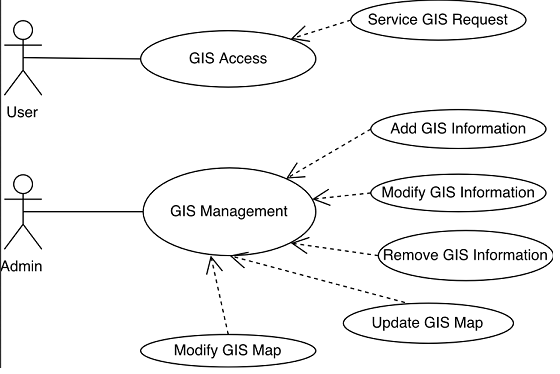
\includegraphics[scale=0.75]{GIS_Use_Case_Diagram.png}
	
	\section{Domain Model}
	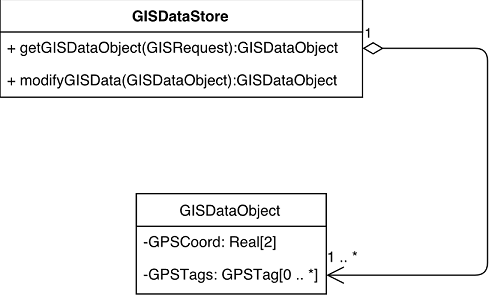
\includegraphics[scale=0.75]{GIS_Domain_Model.png}
	\vspace{0.25cm}\newline\newline
	When thinking of the domain model for the GIS module, it is important to emphasise
	the data storage and retrieval aspects of this module. The GIS module is going to
	persist and service requests for GIS information which forms the basis of the entire
	system. Exploring various techniques such as data warehouses may be options in
	terms of realising the system in finer detail.	
	
	\section{Service Contracts}
	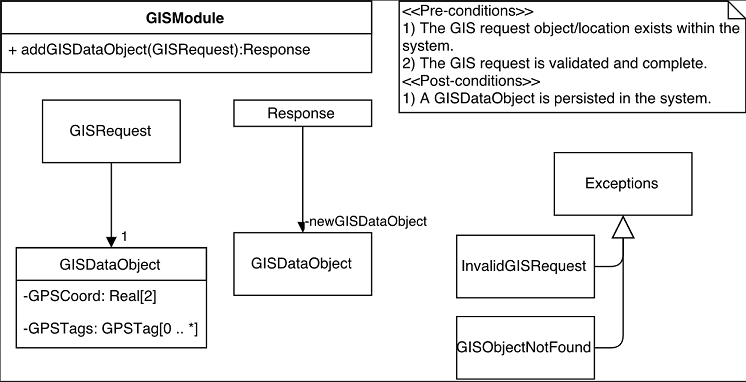
\includegraphics[scale=0.75]{GIS_Service_Contract.png}
	\vspace{0.5cm}\newline
	The service contract specified above will be refused under two conditions. If the GIS
	location or object does not exist or if the request fails the validation protocol, then the
	contract can be refused. Otherwise, the GIS object will be persisted and stored in the
	system. Note that the GIS object storage system is not necessarily dependent on a
	strict coupling to the representation of the GIS object in that the storage system must
	be generic enough such that the objects stored can be changed without extensive
	system reworks.\newline\newline
	Use cases:
	\begin{itemize}
		\item getCurrentLocation: Determine the current location of the device that is used to
		\item access NavUP through services provided in the Data module
	\end{itemize}
		
	
	\section{Technologies - Updated}
	\subsection{waffle.io}
		We decided to use waffle.io to perform standardised project and team management. This was due to the fact that waffle.io is an open source tool that offers a variety of necessary features for project management. It also seamlessly integrates with GitHub and Slack, which we are required to use in this implementation phase. It offers the ability to generate Scrum Boards based on our GitHub issues and pull requests, which it tracks automatically. It gives you the ability to track open issues within your repository, track the issues that are complete, and track the performance of your team on an individual basis. It does this through the visualisation of issues that have the status of either Backlog, Ready, In Progress or Done on an interactive board.
	\subsection{Java}
		There are many reasons why we decided to use Java. One of the main reasons being that is an open source language, which is also very popular, meaning it is heavily maintained and supported. It is also a platform-independent language, meaning it runs regardless of hardware and software.
	\subsection{Mockito}
		We decided to use Mockito as our testing framework as it provides a simple API for creating unit tests for Java. Java and Mockito are very popular in the software development community, which means it is also heavily maintained and supported.
	\subsection{ArcGIS}
		We chose this geographic information system as the base of the GIS module as it provides all the features that are required by a geospatial application. It provides the ability to map data, visual data and analyse data according to the functionality of the application you are developing, whether it is mobile-based, web-based or a standalone application. It also seamlessly integrates with Java, which will be used for the bulk of the application, whilst maintaining scalability and reliability.
	\subsection{ArcMap}
		We chose to use ArcMap for geospatial manipulation as it is an integral tool that is part of ArcGIS. It allows for the creation of maps, the ability to manage mapped data, and the ability to perform analysis on this data. It does this in both 2D and 3D format, providing the user with a truly interactive experience.
\end{document}